\documentclass[]{aiaa-pretty} %submit, draft, journal options can be used
\usepackage[belowskip=0pt, aboveskip=0pt]{subcaption}
\usepackage{float}
\usepackage{caption}
\usepackage{tcolorbox}
%\setlength{\belowcaptionskip}{-10pt}

%\usepackage{classdiagram}
%\usepackage[T1]{fontenc}

\usepackage{amsmath}
\newenvironment{rcases}
  {\left.\begin{aligned}}
  {\end{aligned}\right\rbrace}
\newenvironment{lcases}
  {\left\lbrace\begin{aligned}}
  {\end{aligned}\right.}

\usepackage{amssymb}
\usepackage{amsfonts}
% * <komahan.cool@gmail.com> 2018-04-24T04:09:52.446Z:
%
% > }
%
% ^.
\usepackage{multirow}
\usepackage{booktabs}
\usepackage{doi}
\usepackage{xcolor}
\usepackage{graphicx,dblfloatfix} 
\usepackage{algorithm}
\usepackage{algpseudocode}
%\usepackage[superscript]{cite}
\usepackage[numbers,compress,sort]{natbib}
%
\usepackage{soul,xcolor}
\setstcolor{blue}

% User defined commands
\newcommand{\ds}{\displaystyle}
\newcommand{\mb}{\mathbf}
\newcommand{\mr}{\mathrm}
\newcommand{\mbs}{\boldsymbol}
\newcommand{\f}{\frac}
\newcommand{\p}{\partial}
\newcommand{\vect}[1]{\vec{\mathbf{#1}}}
\newcommand{\ignore}[1]{}

\renewcommand{\pd}[2]{\displaystyle{\dfrac{\partial #1}{\partial #2}}}
\newcommand{\td}[2]{\dfrac{d #1}{d #2}}
\newcommand{\pdt}[2]{\dfrac{\partial^2 #1}{\partial #2^2}}
\newcommand{\tdt}[2]{\dfrac{d^2 #1}{d #2^2}}
\newcommand{\pdtno}[2]{\dfrac{\partial^2 #1}{\partial #2}}
\newcommand{\pdd}[3]{\dfrac{\partial^2 #1}{\partial #2 \partial #3}}
\newcommand{\pff}[3]{\dfrac{d^2 #1}{d #2 d #3}}

% Redefined commands
\renewcommand\floatpagefraction{.95}
\usepackage{cleveref}
\crefname{subsection}{subsection}{subsections}

%\newcommand{\com}[1]{\textcolor{red}{#1}}
\newcommand{\new}[1]{{\leavevmode\color{black}{#1}}}
\newcommand{\kb}[1]{{\leavevmode\color{blue}{#1}}}
\newcommand{\off}[1]{}
\newcommand{\gjk}[1]{{\leavevmode\color{Red}{#1}}}

\usepackage{cmbright}
%\usepackage{arev}
\renewcommand\familydefault{\sfdefault} 

\usepackage{algorithm}
\usepackage{algpseudocode}

\graphicspath{{talk/}{talk/figures/}{figures/}}

\title{Isogeometric Finite Element Analysis using Non-Uniform Rational B-Splines}
\author{Komahan Boopathy  and Siddarth Niranjan Babu\\
  {\normalsize\itshape School of Aerospace Engineering, Georgia Institute of Technology,
    Atlanta, GA, 30332-0150, USA.}\\
} 

\begin{document}
\maketitle


%\abstract{}


\section{Introduction and Motivation}
Non-uniform Rational B-Splines (NURBS) \cite{Piegl:NurbsBook} are a
popular way to represent curves and surfaces in geometry modeling. In
other words, they provide a basis for three-dimensional euclidean
space. In principle, they can be used to span other spaces as well,
for example, N-dimensional vector spaces in finite element
analysis. This realization has led to the development of isogeometric
analysis
(IGA)~\cite{HUGHES20054135,KACPRZYK201487,NGUYEN201589,Agrawal2018,Milic2013}
where the same functions used for geometry representation is also used
to represent displacement field.
\subsection{Importance of IGA}
\begin{itemize}
  \item FEM utilizes the approximate form of CAD geometry by discretizing them into a smaller sub-geometry called elements. Whereas in IGA, CAD-based NURBS described geometries are directly employed in the analysis without making any geometrical approximations like in FEM.
  \item IGA reduces the burden of mesh regeneration and thus minimizes the computational cost. % to a great extent.
  \item Due to inherent higher order continuity and exact representation of geometrical features, IGA has been shown to be advantageous in contact, fluid, structural vibration problems and more. 
  \item IGA can be applied to specific problems which have been solved with FEM to attain improved solution.
\end{itemize}

\section{Framework}
The main objective of the project is implementation of NURBS based Isogeometric Analysis(IGA) within the existing Finite element code architecture. IGA is a recently introduced technique that employs the Computer Aided Design concepts of Non-uniform Rational B-splines(NURBS) tool to bridge the substantial  bottleneck between the CAD and finite element analysis field. The fundamental concept of IGA is to utilize the NURBS basis functions not only for the construction or as a handler of the exact form of CAD geometries, but also as a tool that can be used for their mathematical analysis. To describe the application of IGA, a standard infinite plate with a circular hole problem in tension as shown in Figure~\ref{fig:iga-demo} is chosen. 
\begin{figure}[h] 
  \centering
  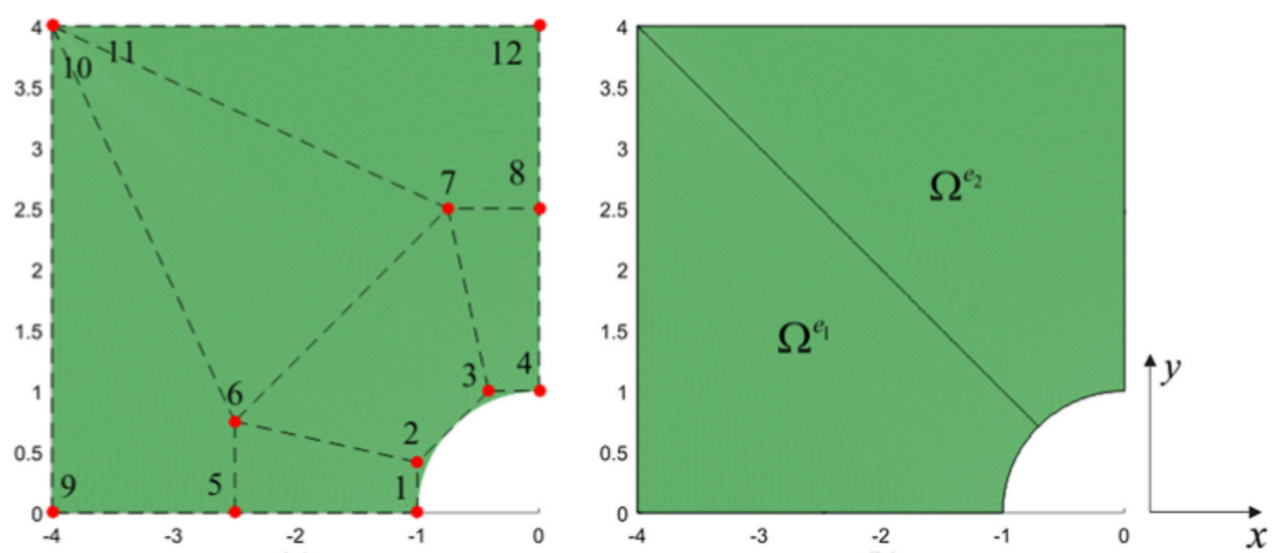
\includegraphics[width=0.5\linewidth]{iga-demo.pdf}
  \caption{\emph{NURBS decretized quarter-plate with a hole}}
  \label{fig:iga-demo}
\end{figure}
In IGA, apart from the geometrical details(length, height, width) of a
model, its parametric details such as knot vectors , the order of
NURBS basis functions, and the control points are also needed to
construct the exact form of discretized geometry. The evaluation of
NURBS basis functions and their respective derivatives, along with
their corresponding mappings are need to be done along with the
enforcement procedure for different boundary conditions for NURBS
defined geometry. The combinations of these complete the processing
stage for the proposed implementation of IGA within the FEA structure.

\section{Results}

\section{Conclusions}
\bibliographystyle{myabbrvnat} 
\bibliography{references}

\end{document}

